\documentclass{standalone}
\usepackage{tikz}
\usetikzlibrary{patterns, positioning}

\begin{document}
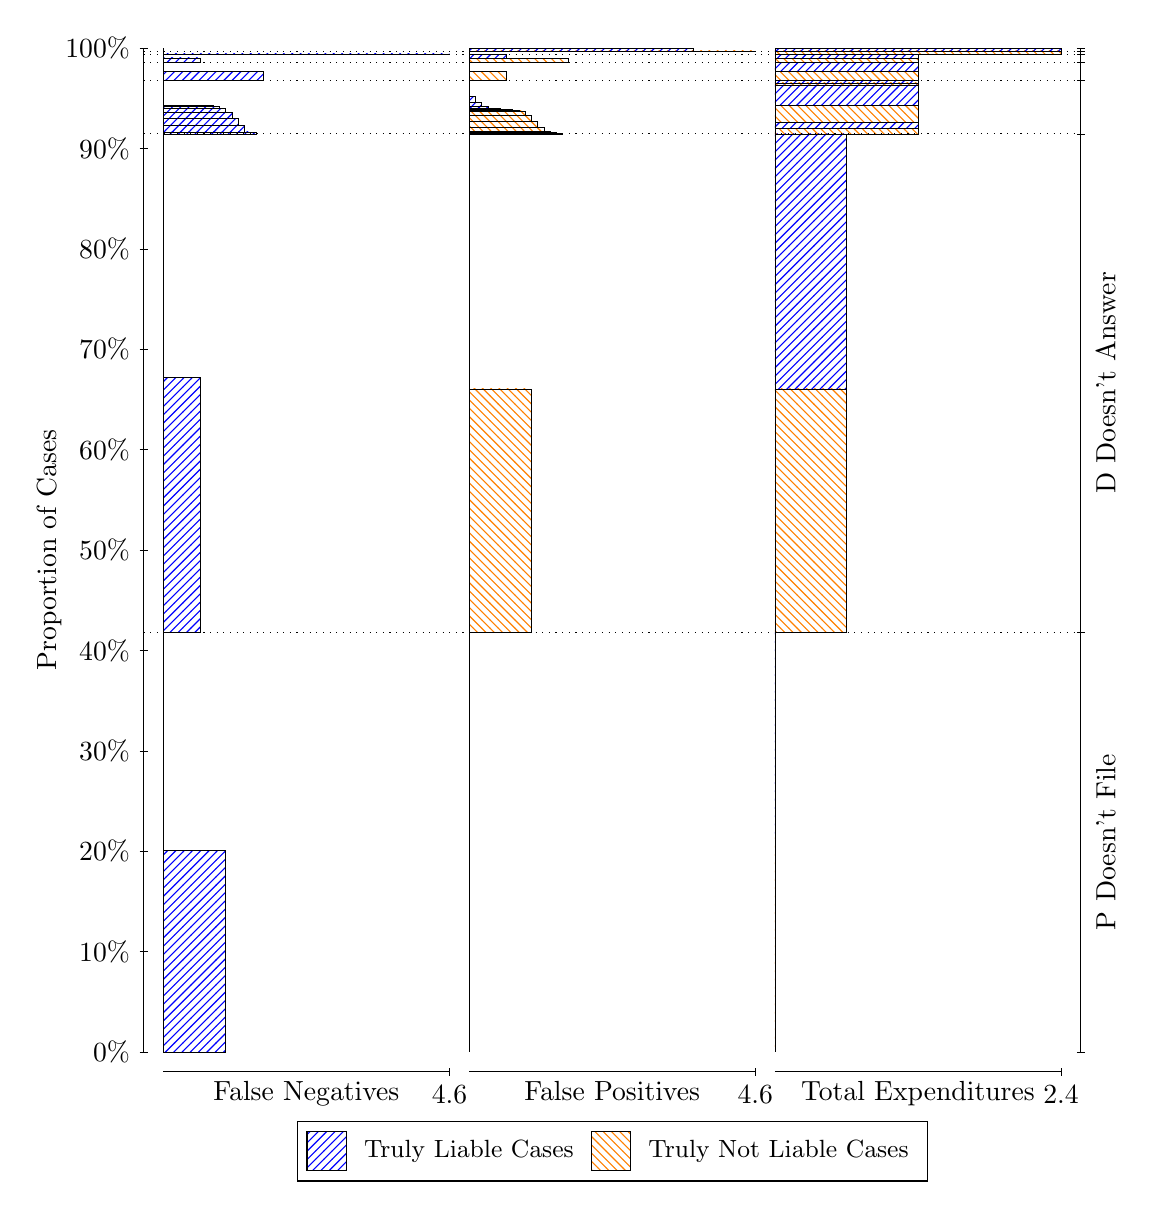
\begin{tikzpicture}
\draw[black, very thin] (1.5,1.75) -- (1.5,14.5);
\node[rotate=90, anchor=center] at (0.3, 8.125) {Proportion of Cases};
\draw[black, very thin] (1.45,1.75) -- (1.55,1.75);
\node[anchor=east] at (1.45, 1.75) {0\%};
\draw[black, very thin] (1.45,3.025) -- (1.55,3.025);
\node[anchor=east] at (1.45, 3.025) {10\%};
\draw[black, very thin] (1.45,4.3) -- (1.55,4.3);
\node[anchor=east] at (1.45, 4.3) {20\%};
\draw[black, very thin] (1.45,5.575) -- (1.55,5.575);
\node[anchor=east] at (1.45, 5.575) {30\%};
\draw[black, very thin] (1.45,6.85) -- (1.55,6.85);
\node[anchor=east] at (1.45, 6.85) {40\%};
\draw[black, very thin] (1.45,8.125) -- (1.55,8.125);
\node[anchor=east] at (1.45, 8.125) {50\%};
\draw[black, very thin] (1.45,9.4) -- (1.55,9.4);
\node[anchor=east] at (1.45, 9.4) {60\%};
\draw[black, very thin] (1.45,10.675) -- (1.55,10.675);
\node[anchor=east] at (1.45, 10.675) {70\%};
\draw[black, very thin] (1.45,11.95) -- (1.55,11.95);
\node[anchor=east] at (1.45, 11.95) {80\%};
\draw[black, very thin] (1.45,13.225) -- (1.55,13.225);
\node[anchor=east] at (1.45, 13.225) {90\%};
\draw[black, very thin] (1.45,14.5) -- (1.55,14.5);
\node[anchor=east] at (1.45, 14.5) {100\%};

\draw[black, very thin] (13.4,1.75) -- (13.4,14.5);
\draw[black, very thin] (13.35,1.75) -- (13.45,1.75);
\node[anchor=west] at (13.35, 1.75) {};
\draw[black, very thin] (13.35,7.0809) -- (13.45,7.0809);
\node[anchor=west] at (13.35, 7.0809) {};
\draw[black, very thin] (13.35,13.411) -- (13.45,13.411);
\node[anchor=west] at (13.35, 13.411) {};
\draw[black, very thin] (13.35,14.086) -- (13.45,14.086);
\node[anchor=west] at (13.35, 14.086) {};
\draw[black, very thin] (13.35,14.317) -- (13.45,14.317);
\node[anchor=west] at (13.35, 14.317) {};
\draw[black, very thin] (13.35,14.422) -- (13.45,14.422);
\node[anchor=west] at (13.35, 14.422) {};
\draw[black, very thin] (13.35,14.461) -- (13.45,14.461);
\node[anchor=west] at (13.35, 14.461) {};
\draw[black, very thin] (13.35,14.5) -- (13.45,14.5);
\node[anchor=west] at (13.35, 14.5) {};

\draw[black, very thin, pattern color=blue, pattern=north east lines] (1.75,1.75) rectangle (2.5399,4.3121);
\draw[black, very thin, pattern color=orange, pattern=north west lines] (1.75,4.3121) rectangle (1.75,7.0809);
\draw[black, very thin, pattern color=blue, pattern=north east lines] (1.75,7.0809) rectangle (2.2239,10.321);
\draw[black, very thin, pattern color=orange, pattern=north west lines] (1.75,10.321) rectangle (1.75,13.411);
\draw[black, very thin, pattern color=blue, pattern=north east lines] (1.75,13.411) rectangle (2.9348,13.424);
\draw[black, very thin, pattern color=blue, pattern=north east lines] (1.75,13.424) rectangle (2.8558,13.435);
\draw[black, very thin, pattern color=blue, pattern=north east lines] (1.75,13.435) rectangle (2.7768,13.518);
\draw[black, very thin, pattern color=blue, pattern=north east lines] (1.75,13.518) rectangle (2.6978,13.61);
\draw[black, very thin, pattern color=blue, pattern=north east lines] (1.75,13.61) rectangle (2.6188,13.684);
\draw[black, very thin, pattern color=blue, pattern=north east lines] (1.75,13.684) rectangle (2.5399,13.738);
\draw[black, very thin, pattern color=blue, pattern=north east lines] (1.75,13.738) rectangle (2.4609,13.759);
\draw[black, very thin, pattern color=blue, pattern=north east lines] (1.75,13.759) rectangle (2.3819,13.767);
\draw[black, very thin, pattern color=blue, pattern=north east lines] (1.75,13.767) rectangle (2.3029,13.773);
\draw[black, very thin, pattern color=orange, pattern=north west lines] (1.75,13.773) rectangle (1.75,14.086);
\draw[black, very thin, pattern color=blue, pattern=north east lines] (1.75,14.086) rectangle (3.0138,14.2);
\draw[black, very thin, pattern color=orange, pattern=north west lines] (1.75,14.2) rectangle (1.75,14.317);
\draw[black, very thin, pattern color=blue, pattern=north east lines] (1.75,14.317) rectangle (2.2239,14.375);
\draw[black, very thin, pattern color=orange, pattern=north west lines] (1.75,14.375) rectangle (1.75,14.422);
\draw[black, very thin, pattern color=blue, pattern=north east lines] (1.75,14.422) rectangle (5.3833,14.425);
\draw[black, very thin, pattern color=orange, pattern=north west lines] (1.75,14.425) rectangle (1.75,14.461);
\draw[black, very thin, pattern color=orange, pattern=north west lines] (1.75,14.461) rectangle (1.75,14.463);
\draw[black, very thin, pattern color=blue, pattern=north east lines] (1.75,14.463) rectangle (1.75,14.5);
\draw[black, very thin, pattern color=orange, pattern=north west lines] (5.6333,1.75) rectangle (5.6333,4.5188);
\draw[black, very thin, pattern color=blue, pattern=north east lines] (5.6333,4.5188) rectangle (5.6333,7.0809);
\draw[black, very thin, pattern color=orange, pattern=north west lines] (5.6333,7.0809) rectangle (6.4232,10.171);
\draw[black, very thin, pattern color=blue, pattern=north east lines] (5.6333,10.171) rectangle (5.6333,13.411);
\draw[black, very thin, pattern color=orange, pattern=north west lines] (5.6333,13.411) rectangle (6.8181,13.417);
\draw[black, very thin, pattern color=orange, pattern=north west lines] (5.6333,13.417) rectangle (6.7391,13.424);
\draw[black, very thin, pattern color=orange, pattern=north west lines] (5.6333,13.424) rectangle (6.6601,13.445);
\draw[black, very thin, pattern color=orange, pattern=north west lines] (5.6333,13.445) rectangle (6.5812,13.494);
\draw[black, very thin, pattern color=orange, pattern=north west lines] (5.6333,13.494) rectangle (6.5022,13.565);
\draw[black, very thin, pattern color=orange, pattern=north west lines] (5.6333,13.565) rectangle (6.4232,13.644);
\draw[black, very thin, pattern color=orange, pattern=north west lines] (5.6333,13.644) rectangle (6.3442,13.701);
\draw[black, very thin, pattern color=orange, pattern=north west lines] (5.6333,13.701) rectangle (6.2652,13.709);
\draw[black, very thin, pattern color=orange, pattern=north west lines] (5.6333,13.709) rectangle (6.1862,13.724);
\draw[black, very thin, pattern color=blue, pattern=north east lines] (5.6333,13.724) rectangle (6.0283,13.731);
\draw[black, very thin, pattern color=blue, pattern=north east lines] (5.6333,13.731) rectangle (5.9493,13.739);
\draw[black, very thin, pattern color=blue, pattern=north east lines] (5.6333,13.739) rectangle (5.8703,13.759);
\draw[black, very thin, pattern color=blue, pattern=north east lines] (5.6333,13.759) rectangle (5.7913,13.813);
\draw[black, very thin, pattern color=blue, pattern=north east lines] (5.6333,13.813) rectangle (5.7123,13.887);
\draw[black, very thin, pattern color=blue, pattern=north east lines] (5.6333,13.887) rectangle (5.6333,14.086);
\draw[black, very thin, pattern color=orange, pattern=north west lines] (5.6333,14.086) rectangle (6.1072,14.204);
\draw[black, very thin, pattern color=blue, pattern=north east lines] (5.6333,14.204) rectangle (5.6333,14.317);
\draw[black, very thin, pattern color=orange, pattern=north west lines] (5.6333,14.317) rectangle (6.8971,14.364);
\draw[black, very thin, pattern color=blue, pattern=north east lines] (5.6333,14.364) rectangle (6.1072,14.422);
\draw[black, very thin, pattern color=orange, pattern=north west lines] (5.6333,14.422) rectangle (5.6333,14.458);
\draw[black, very thin, pattern color=blue, pattern=north east lines] (5.6333,14.458) rectangle (5.6333,14.461);
\draw[black, very thin, pattern color=orange, pattern=north west lines] (5.6333,14.461) rectangle (9.2667,14.463);
\draw[black, very thin, pattern color=blue, pattern=north east lines] (5.6333,14.463) rectangle (8.4768,14.5);
\draw[black, very thin, pattern color=orange, pattern=north west lines] (9.5167,1.75) rectangle (9.5167,4.5188);
\draw[black, very thin, pattern color=blue, pattern=north east lines] (9.5167,4.5188) rectangle (9.5167,7.0809);
\draw[black, very thin, pattern color=orange, pattern=north west lines] (9.5167,7.0809) rectangle (10.425,10.171);
\draw[black, very thin, pattern color=blue, pattern=north east lines] (9.5167,10.171) rectangle (10.425,13.411);
\draw[black, very thin, pattern color=orange, pattern=north west lines] (9.5167,13.411) rectangle (11.333,13.482);
\draw[black, very thin, pattern color=blue, pattern=north east lines] (9.5167,13.482) rectangle (11.333,13.556);
\draw[black, very thin, pattern color=orange, pattern=north west lines] (9.5167,13.556) rectangle (11.333,13.77);
\draw[black, very thin, pattern color=blue, pattern=north east lines] (9.5167,13.77) rectangle (11.333,14.031);
\draw[black, very thin, pattern color=orange, pattern=north west lines] (9.5167,14.031) rectangle (11.333,14.058);
\draw[black, very thin, pattern color=blue, pattern=north east lines] (9.5167,14.058) rectangle (11.333,14.086);
\draw[black, very thin, pattern color=orange, pattern=north west lines] (9.5167,14.086) rectangle (11.333,14.204);
\draw[black, very thin, pattern color=blue, pattern=north east lines] (9.5167,14.204) rectangle (11.333,14.317);
\draw[black, very thin, pattern color=orange, pattern=north west lines] (9.5167,14.317) rectangle (11.333,14.364);
\draw[black, very thin, pattern color=blue, pattern=north east lines] (9.5167,14.364) rectangle (11.333,14.422);
\draw[black, very thin, pattern color=orange, pattern=north west lines] (9.5167,14.422) rectangle (13.15,14.458);
\draw[black, very thin, pattern color=blue, pattern=north east lines] (9.5167,14.458) rectangle (13.15,14.461);
\draw[black, very thin, pattern color=orange, pattern=north west lines] (9.5167,14.461) rectangle (13.15,14.463);
\draw[black, very thin, pattern color=blue, pattern=north east lines] (9.5167,14.463) rectangle (13.15,14.5);
\draw[black, dotted] (1.5,7.0809) -- (13.4,7.0809);
\draw[black, dotted] (1.5,13.411) -- (13.4,13.411);
\draw[black, dotted] (1.5,14.086) -- (13.4,14.086);
\draw[black, dotted] (1.5,14.317) -- (13.4,14.317);
\draw[black, dotted] (1.5,14.422) -- (13.4,14.422);
\draw[black, dotted] (1.5,14.461) -- (13.4,14.461);
\draw[black, very thin] (1.75,1.5) -- (5.3833,1.5);
\node[anchor=north] at (3.5667, 1.5) {False Negatives};
\draw[black, very thin] (5.3833,1.45) -- (5.3833,1.55);
\node[anchor=north] at (5.3833, 1.45) {4.6};

\draw[black, very thin] (5.6333,1.5) -- (9.2667,1.5);
\node[anchor=north] at (7.45, 1.5) {False Positives};
\draw[black, very thin] (9.2667,1.45) -- (9.2667,1.55);
\node[anchor=north] at (9.2667, 1.45) {4.6};

\draw[black, very thin] (9.5167,1.5) -- (13.15,1.5);
\node[anchor=north] at (11.333, 1.5) {Total Expenditures};
\draw[black, very thin] (13.15,1.45) -- (13.15,1.55);
\node[anchor=north] at (13.15, 1.45) {2.4};

\node[black, centered, rotate=90] at (13.72, 4.4155) {P Doesn't File};
\node[black, centered, rotate=90] at (13.72, 10.246) {D Doesn't Answer};






\draw (7.449999999999999,1.5) node[draw=none] (baseCoordinate) {};
\begin{scope}[align=center]
        \matrix[scale=0.5, draw=black, below=0.5cm of baseCoordinate, nodes={draw}, column sep=0.1cm]{
            \node[rectangle, draw, minimum width=0.5cm, minimum height=0.5cm, pattern=north east lines, pattern color=blue] {}; &
            \node[draw=none, font=\small] (B) {Truly Liable Cases}; &
            \node[rectangle, draw, minimum width=0.5cm, minimum height=0.5cm, pattern=north west lines, pattern color=orange] {}; &
            \node[draw=none, font=\small] (B) {Truly Not Liable Cases}; \\
            };
\end{scope}

\end{tikzpicture}
\end{document}